\chapter{Estudo de Caso}
\label{cap:proposta}

Nos capítulos anteriores foram apresentas algumas tecnologias importantes para a implementação de aplicações que se encaixam no contexto Big Data. O propósito desta etapa inicial consistiu em levantar o conhecimento necessário para que seja possível analisar e projetar soluções baseadas em diferentes cenários que envolvem o processamento de grandes volumes de dados. O próximo passo deste trabalho é aplicar os conceitos vistos até o momento em um estudo de caso real. Portanto o objetivo deste capítulo é propor um modelo de arquitetura que deverá ser projetado e construído na sequência desta pesquisa.

\section{Motivação}

Com o surgimento de políticas públicas voltadas para transparência digital, principalmente após o estabelecimento da Lei de Acesso à Informação\footnote{\url{http://www.planalto.gov.br/ccivil_03/_ato2011-2014/2011/lei/l12527.htm}}, a população brasileira tem exercido um papel fundamental no monitoramento das atividades do governo federal. A realização de eventos como a maratona Hackathon\footnote{\url{http://www2.camara.leg.br/responsabilidade-social/edulegislativa/educacao-legislativa-1/educacao-para-a-democracia-1/hackathon/hackathon}} da Câmara dos Deputados contribui e incentiva ainda mais a adesão da comunidade de desenvolvedores para a construção de softwares voltados para este contexto.

As redes sociais também desempenham uma função essencial neste processo. Este meio de comunicação deixou de ser utilizado apenas para lazer e atualmente é usado pelos cidadãos para expressar opiniões dos mais variados assuntos, princialmente quando refere-se a questões políticas e sociais aplicadas no país.

\section{Problema}

A política brasileira vem sendo bastante criticada nos últimos anos, escândalos políticos, notícias frequentes sobre corrupção, serviços públicos de má qualidade, entre outros fatores, contribuem para a insatisfação do cidadão brasileiro em relação ao governo do país. Tendo em vista que as redes sociais são utilizadas por grande parcela da população como meio para expressar suas opiniões, uma análise minuciosa destas informações pode ser um fator de extrema importância para revelar os principais motivos que geram esse descontentamento. Processar estas informações não é uma tarefa trivial, pois os dados gerados por este meio podem estar na ordem de terabytes.

\section{Arquitetura}

Nesta seção será apresentado um modelo de aplicação para solucionar o problema descrito anteriormente. A quantidade de dados gerados por redes sociais exige uma abordagem voltada para o contexto Big Data, pois como mostrado nos capítulos anteriores, bancos de dados relacionais e outras tecnologias tradicionais não são adequadas para este tipo de problema. Portanto o estudo de caso proposto por este trabalho tem como objetivo a construção de uma aplicação que realize análise de dados de redes sociais voltados para políticas públicas. Resumidamente o sistema deverá ser capaz de executar as seguintes atividades:

\begin{itemize}
  \item Extrair mensagens relacionadas a políticas públicas postadas por usuários de redes sociais.
  \item Prover escalabilidade linear para a quantidade de registros que são armazenados.
  \item Analisar as publicações e classificá-las de acordo com o conteúdo.
  \item Exibir para o usuário final uma interface \textit{web} para visualização dos resultados obtidos após a análise.
\end{itemize}

A figura \ref{fig-proposta} apresenta o modelo de arquitetura que será adotado pela solução proposta neste trabalho. 

\begin{figure}[ht!]
	\centering
	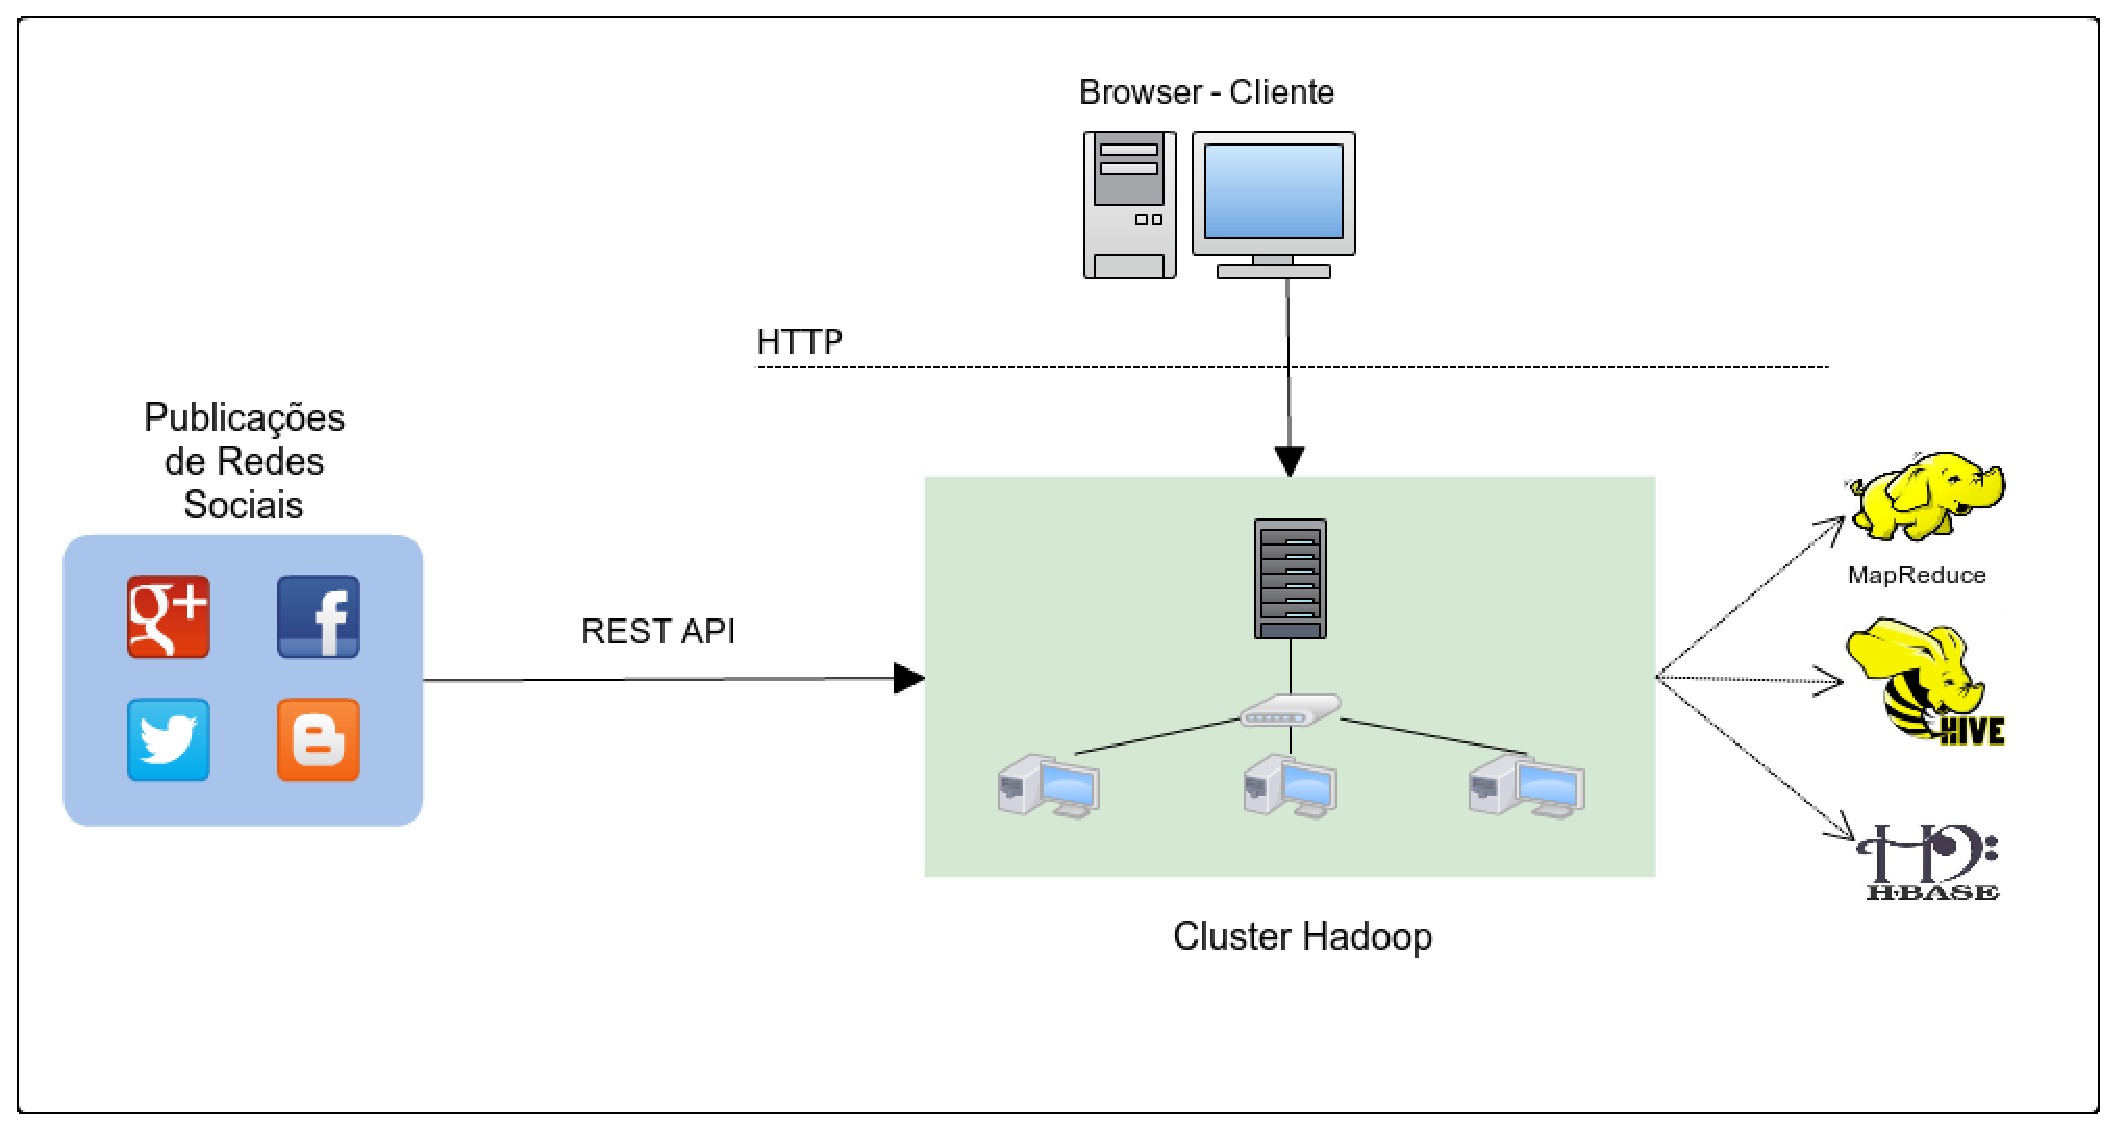
\includegraphics[keepaspectratio=true,scale=0.35]
	  {figuras/proposta.eps}
	\caption[Arquitetura da solução]{Arquitetura da solução
	\protect\linebreak Fonte: Autor}
	\label{fig-proposta}
\end{figure}
\FloatBarrier

A extração de publicações das redes sociais deverá ocorrer através das APIs disponibilizadas pelas redes sociais Facebook\footnote{\url{https://developers.facebook.com/docs/graph-api/quickstart/v2.0}}, Twitter\footnote{\url{https://dev.twitter.com/docs/streaming-apis/streams/public}} e YouTube\footnote{\url{https://developers.google.com/youtube/2.0/developers_guide_protocol_comments}}. Todas estas ferramentas possibilitam capturar postagens públicas através de serviços REST\footnote{\url{http://pt.wikipedia.org/wiki/REST}}. Estas informações devem ser armazenadas e analisadas em um \textit{cluster} Hadoop. Os resultados obtidos pela análise serão disponibilizados através de um serviço \textit{web}.

O processo de análise das mensagens que estarão armazenadas no \textit{cluster} ainda está sendo definido. Até o momento, o único método pesquisado procura identificar os sentimentos que um determinado usuário expressa em suas mensagens de redes sociais, este modelo é definido como análise de sentimentos. \citeonline{araujo2013} destacaram abordagens para análise de sentimentos em postagens retiradas de redes sociais. Algumas delas são apresentadas a seguir:

\begin{itemize}

  \item \textbf{Emoticons\footnote{Sequencia de caracteres tipográficos que expressam emoções.}:} Análise baseada na presença de \textit{emoticons} na corpo da sentença. Uma das abordagens mais ineficientes, segundo \citeonline{araujo2013}.
  \item \textbf{LIWC(Linguistic Inquiry and Word Count):} Ferramenta comercial que utiliza um dicionário de palavras separadas em categorias para estimar os componentes emocionais, cognitivos e estruturais de um texto.
  \item \textbf{SentiStrength:} Utiliza métodos baseados em aprendizado de máquinas, na qual compara métodos de classificação supervisionadas com não supervisionadas.
  \item \textbf{SentiWordNet:} Este método calcula três índices (positivo, negativo, neutro) que indicam o grau – variando de 0 a 1 – de cada um destes sentimentos presentes no texto. Utiliza um dicionário léxico WordNet\footnote{\url{http://wordnet.princeton.edu/}} e aprendizagem de máquina semi-supervisionada.
  \item \textbf{SenticNet:} Método para mineração de opinião e análise de sentimentos que explora técnicas de Inteligência Artificial e Web Semântica.
  \item \textbf{SASA:} Ferramenta \textit{open-source} que se baseia em aprendizado de máquina.

\end{itemize}


















